\documentclass[main.tex]{subfiles}

\begin{document}

\section{Gestion de projet}

\subsection{L’équipe}

\quad L’équipe suit une méthodologie itérative, avec des vérifications régulières pour assurer le suivi de l’avancement et la résolution des problèmes techniques. Chaque étudiant est responsable d’une partie du développement mais doit collaborer avec les autres pour assurer la bonne intégration des sous-systèmes.\\
Les décisions techniques sont prises collectivement, en s’appuyant sur les recommandations des enseignants encadrants et les exigences définies dans le cahier des charges.

En plus du développement technique, l’équipe est chargée de :

\begin{itemize}
	\item Rédiger la documentation technique et le rapport de projet.
	\item Assurer la gestion des versions et des tests.
	\item Préparer la soutenance finale.
\end{itemize}

Ce travail d’équipe permet de garantir une répartition équilibrée des tâches et une réalisation efficace du projet.


\subsection{Diagramme d’éxigence (CDC)}

\begin{figure}[H]
	\centering
	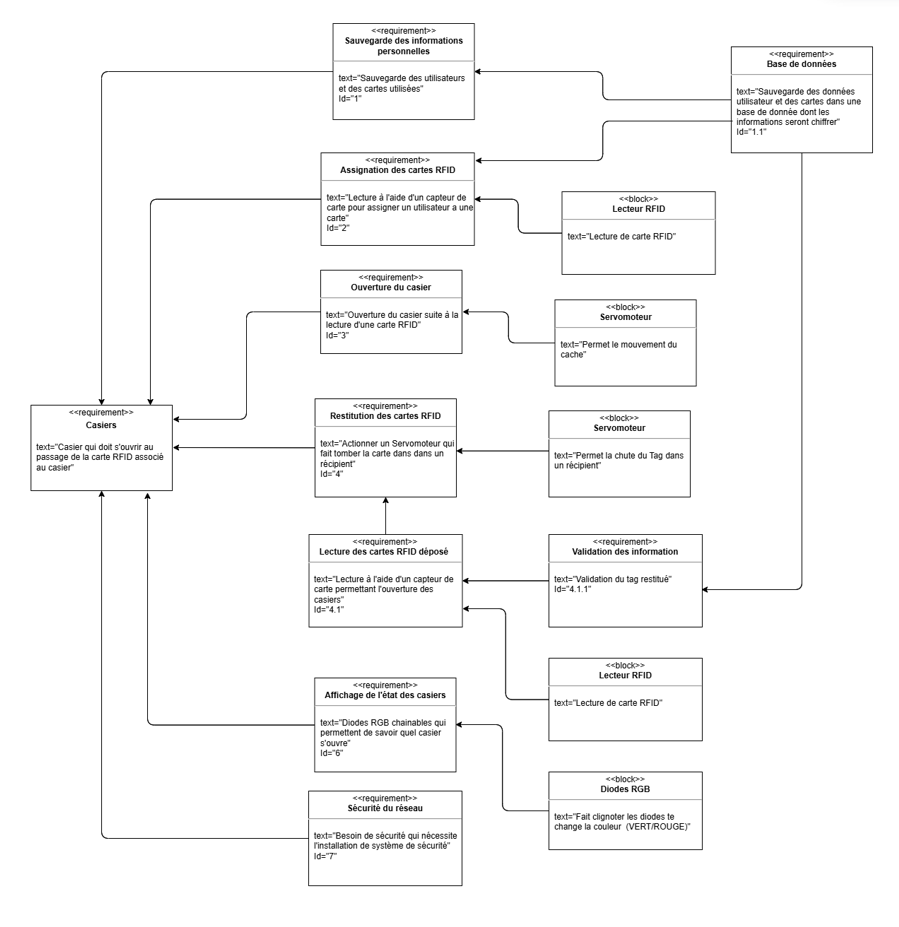
\includegraphics[width=0.8\textwidth]{../images/Diagramme_exigence}
	\caption{Diagramme d'éxigence}
	\label{fig:DDE}
\end{figure}

\subsection{Diagramme de cas d’utilisation}

\begin{figure}[H]
	\centering
	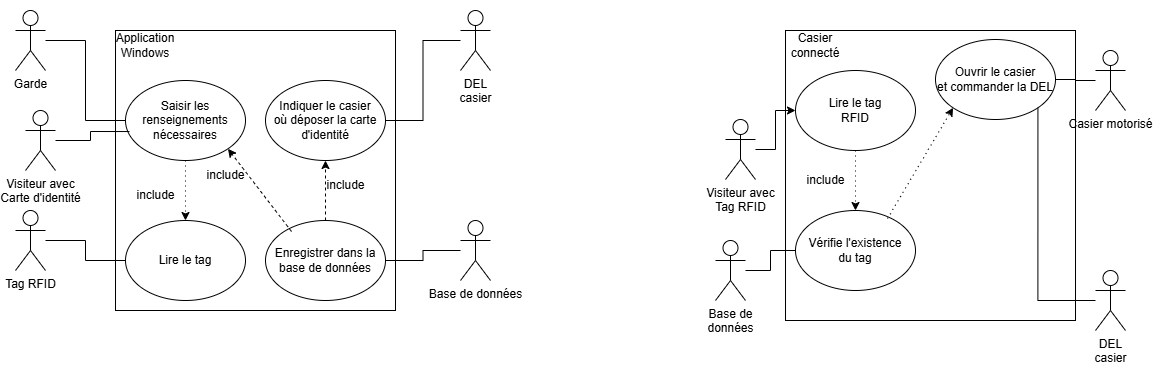
\includegraphics[width=1\textwidth]{../images/DiagrammesUtilisation}
	\caption{Diagramme de cas d’utilisation}
	\label{fig:DDCU}
\end{figure}

\subsection{Diagramme de classe}

\begin{figure}[H]
	\centering
	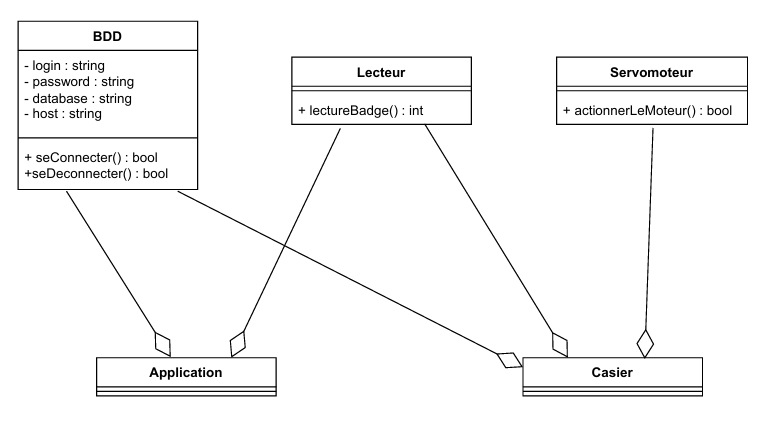
\includegraphics[width=0.7\textwidth]{../images/DiagrammeDeClasseGlobal}
	\caption{Diagramme de classe}
	\label{fig:DDCG}
\end{figure}

\subsection{Base de données (MCD)}

\begin{figure}[H]
	\centering
	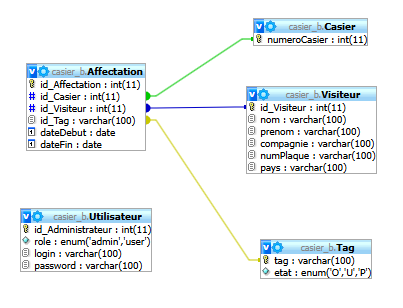
\includegraphics[width=0.7\textwidth]{../images/Base_de_donnee}
	\caption{Base de données}
	\label{fig:BDD}
\end{figure}

\subsection{Diagrammes de séquences}

\begin{figure}[H]
	\centering
	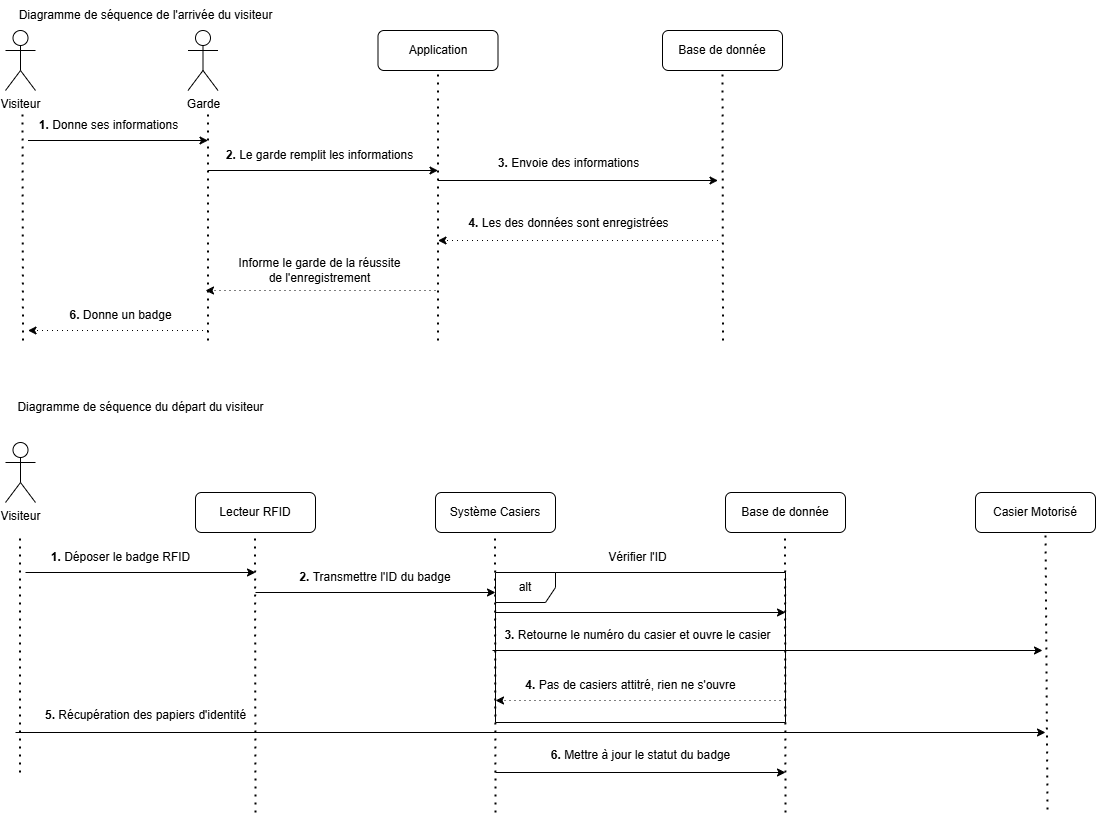
\includegraphics[width=0.9\textwidth]{../images/Diagrammes-Séquence}
	\caption{Diagramme de séquences}
	\label{fig:DDS}
\end{figure}

\subsection{Diagramme de déploiement}

\begin{figure}[H]
	\centering
	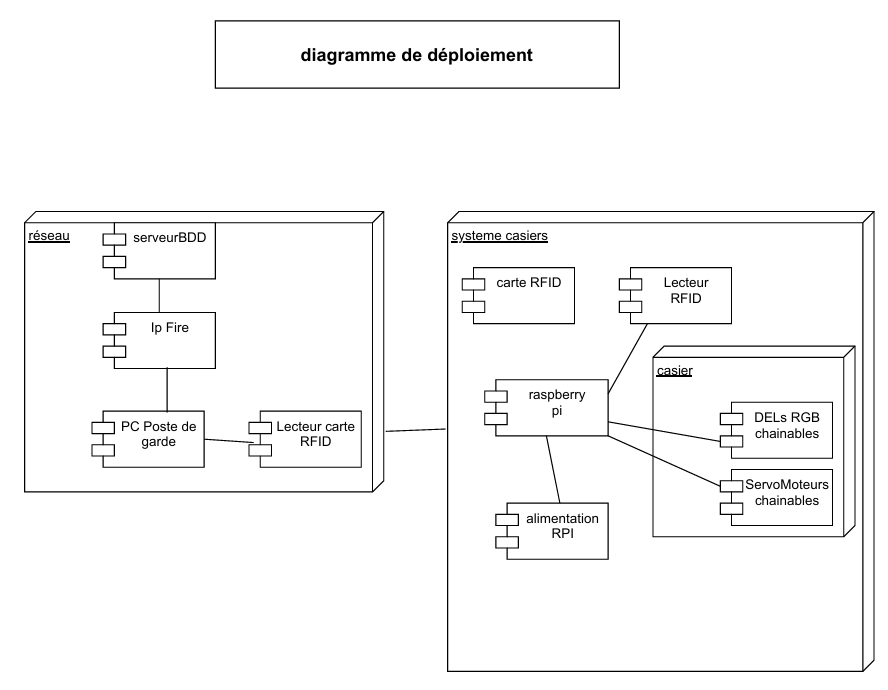
\includegraphics[width=0.8\textwidth]{../images/DiagrammeDeDeploiment}
	\caption{Diagramme de déploiement}
	\label{fig:DDD}
\end{figure}

\subsection{Diagramme de prototype d’IHM (Application Windows)}

\begin{figure}[H]
	\centering
	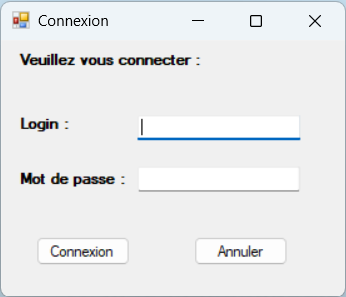
\includegraphics[width=0.6\textwidth]{../images/ConnexionIHM}
	\caption{Page de connexion de l'application}
	\label{fig:PC_APP}
\end{figure}

\begin{figure}[H]
	\centering
	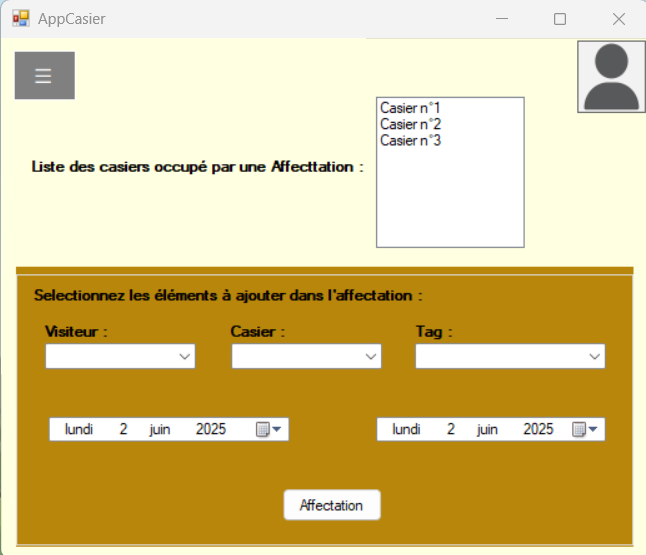
\includegraphics[width=0.7\textwidth]{../images/MainFormIHM}
	\caption{Page d'accueil de l'application}
	\label{fig:PA_APP}
\end{figure}

\begin{figure}[H]
	\centering
	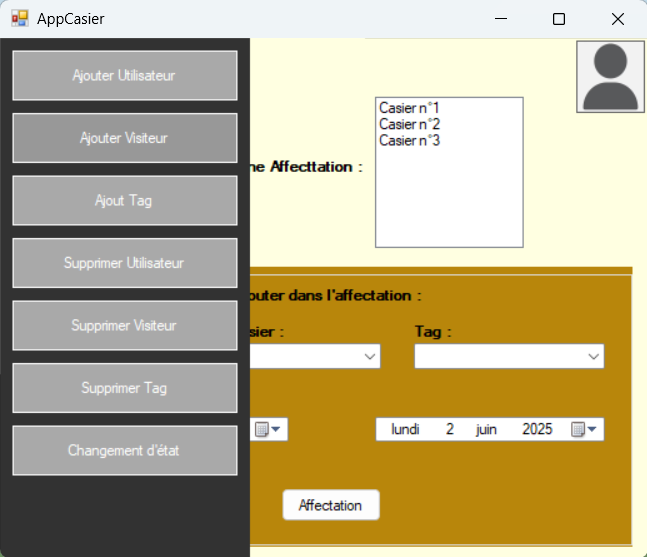
\includegraphics[width=0.7\textwidth]{../images/MenuIHM}
	\caption{Affichage du menu de l'application}
	\label{fig:PAM_APP}
\end{figure}
 
\begin{figure}[H]
	\centering
	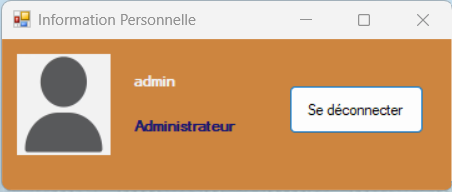
\includegraphics[width=0.7\textwidth]{../images/DecoIHM}
	\caption{Page de déconnexion}
	\label{fig:PD_APP}
\end{figure}

\begin{figure}[H]
	\centering
	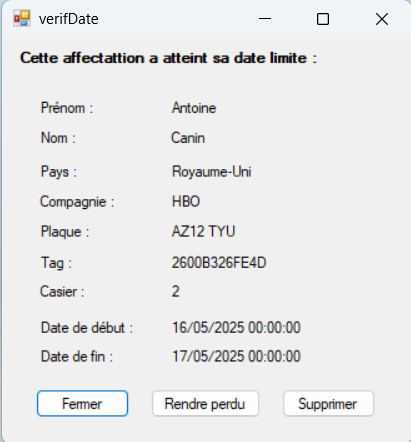
\includegraphics[width=0.7\textwidth]{../images/VerifDateIHM}
	\caption{Page de vérification des dates}
	\label{fig:}
\end{figure}

\begin{figure}[H]
	\centering
	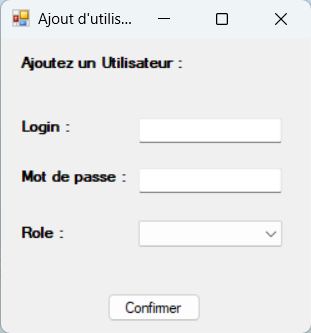
\includegraphics[width=0.6\textwidth]{../images/AjoutUserIHM}
	\caption{Page d'ajout d'utilisateur}
	\label{fig:PAU_APP}
\end{figure}

\begin{figure}[H]
	\centering
	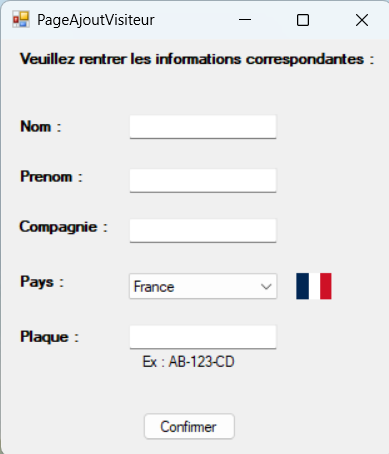
\includegraphics[width=0.6\textwidth]{../images/AjoutVisiteurIHM}
	\caption{Page d'ajout de visiteur}
	\label{fig:PAV_APP}
\end{figure}

\begin{figure}[H]
	\centering
	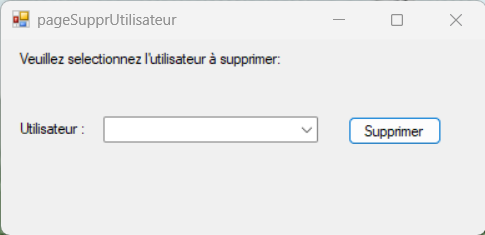
\includegraphics[width=0.7\textwidth]{../images/SupprUserIHM}
	\caption{Page de suppression d'utilisateurs}
	\label{fig:PSU_APP}
\end{figure}

\begin{figure}[H]
	\centering
	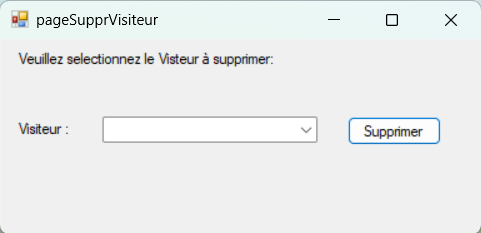
\includegraphics[width=0.7\textwidth]{../images/SupprVisiteurIHM}
	\caption{Page de suppression des visiteurs}
	\label{fig:PSV_APP}
\end{figure}

\begin{figure}[H]
	\centering
	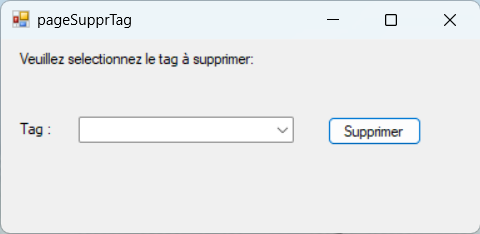
\includegraphics[width=0.7\textwidth]{../images/SupprTagIHM}
	\caption{Page de suppression des tags}
	\label{fig:PST_APP}
\end{figure}

\begin{figure}[H]
	\centering
	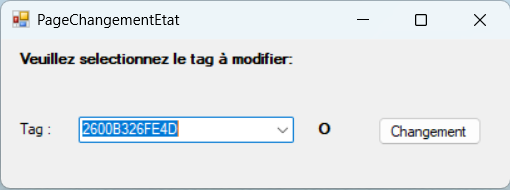
\includegraphics[width=0.7\textwidth]{../images/StateIHM}
	\caption{Page de changement d'état}
	\label{fig:PCE_APP}
\end{figure}

\subsection{Diagramme de Gantt prévisionnel}

\begin{figure}[H]
	\centering
	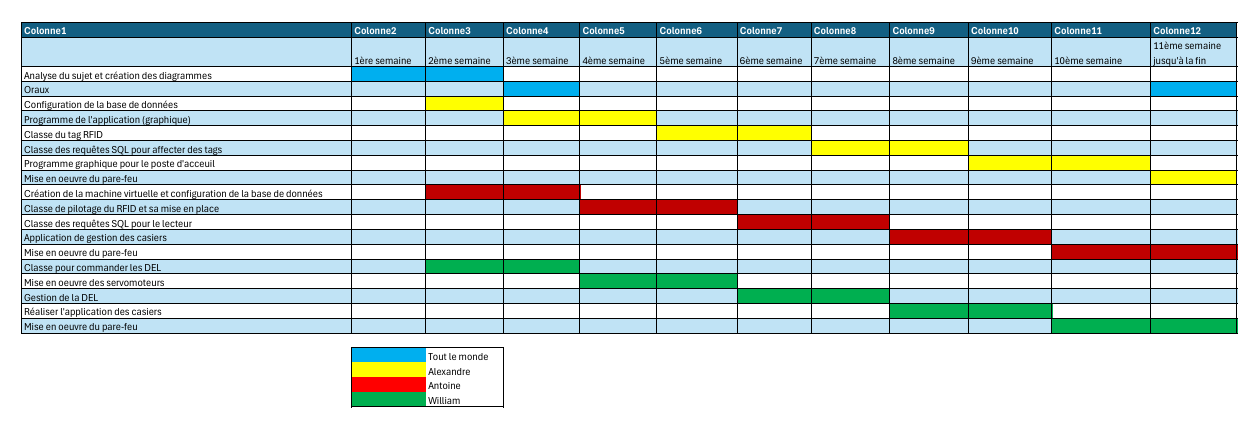
\includegraphics[width=0.9\textwidth]{../images/DiagrammeDeGantP}
	\caption{Diagramme de Gantt prévisionnel}
	\label{fig:DDGP}
\end{figure}

\subsection{Diagramme de Gantt Définitif}

\begin{figure}[H]
	\centering
	\includegraphics[width=1\textwidth]{../images/GanttDef}
	\caption{Diagramme de Gantt définitif}
	\label{fig:DDGP}
\end{figure}

\newpage

\end{document}